\documentclass[a4paper,oneside,twocolumn,notitlepage,dvipdfmx]{jsarticle}
\usepackage[utf8]{inputenc}
\usepackage{amsmath}
\usepackage{amsfonts}
\usepackage{amssymb}
\usepackage{makeidx}
\usepackage{graphicx}
\usepackage{color}
\usepackage{sample}
\usepackage{url}
\usepackage{listings,jlisting}
\setlength\abovecaptionskip{1pt}
\def\baselinestretch{0.3}


\lstset{
  basicstyle={\ttfamily},
  identifierstyle={\small},
  commentstyle={\smallitshape},
  keywordstyle={\small\bfseries},
  ndkeywordstyle={\small},
  stringstyle={\small\ttfamily},
  frame={tb},
  breaklines=true,
  columns=[l]{fullflexible},
  numbers=left,
  xrightmargin=0zw,
  xleftmargin=3zw,
  numberstyle={\scriptsize},
  stepnumber=1,
  numbersep=1zw,
  lineskip=-0.5ex
}

% 以下内容

\student{谷澤 悠太}
\date{令和6年2月5日}
\prof{滝沢 寛之}
\title{ウェブインタフェースを介したスーパーコンピュータ利用環境に関する研究}
%\author{Maohua Zhu, Tao Zhang, Zhenyu Gu, Yuan Xie}
%\journal{MICRO-52, October 12-16, 2019, Columbus, OH, USA}
\nendo{令和5年度}
 
\begin{document}
\maketitle
\section{背景}
近年,高性能計算(High Performance Computing, HPC)システムの用途は多様化し,専門知識を持たない利用者が容易にHPCシステムを利用する需要が高まっている.ただし,このようなユーザは,コマンド操作に基づいた利用環境や,利用するHPCシステムごとに異なる操作方法を使いこなすために多くの学習時間を費やす必要がある.
そこで,従来のコマンド操作に基づく利用環境や,システムごとに異なる利用方法を利用者から隠蔽し,ウェブブラウザを用いて容易かつ統一的にHPCシステムを利用するための研究開発が行われている.\par

\section{課題}
代表的な既存研究として,Open OnDemand (OOD)が挙げられる\cite{citation_2}\cite{citation_3}.OODはウェブインタフェースを介してHPCシステムを利用できる環境を提供する.ユーザはOODのポータルサイトでURL,ユーザ名,パスワードを用いることで,コマンド操作を介さずにジョブの管理を行うことが可能となった.また,世界的に使われている主要なジョブスケジューラ(Tourqe,Slurm,PBS Pro,LSFなど)をサポートすることでシステム間の利用方法の差異も隠蔽している.
ただし,OODがサポートしていないジョブスケジューラで運用されているHPCシステムの場合,OODを利用するためにはOOD自体を改修する必要がある.
例えば,富岳で使われているジョブスケジューラ(Fujitsu Technical Computing Suite, TCS)がOODでサポートされていなかったことから,中尾らはOODをTCS向けに改修した事例を報告している\cite{citation_1}.
その結果,TCSサポートがOOD本体に組み込まれることになったが,他にも様々なジョブスケジューラが存在し,今後も登場することを考えると,ジョブスケジューラの種類が増えるごとにOOD本体を直接修正していく方法には保守性に問題がある.\par

\section{目的}
本研究の目的は,HPC利用者にウェブインターフェスを提供する機能(ウェブ機能)と,ジョブスケジューラ間の差異を抽象化する機能(スケジューラ抽象化機能)を切り分け,それぞれ独立に保守できる構成を実現することである.このために,本研究ではウェブ機能からは統一的にシステムを利用し,スケジューラ抽象化機能でシステム間の差異を埋める構成の利用環境を提案する.この提案手法の模式図を図\ref{fig1}に示す.フロントエンドでは,ユーザはウェブ機能のみとやり取りを行い,ユーザ情報を管理する外部の認証用ディレクトリを用いて安全にHPCシステムを利用することができる.バックエンドでは,ウェブ機能から得られた様々なスケジューラに対するリクエストはスケジューラ抽象化機能が受け取り,処理を行う.この実現のためには,ウェブ機能とスケジューラ抽象化機能を連携させる必要があることから,両者間に求められる情報のやり取りを整理し,適切な連携方法を検討する.\par

\begin{figure}[h]
  \centering
  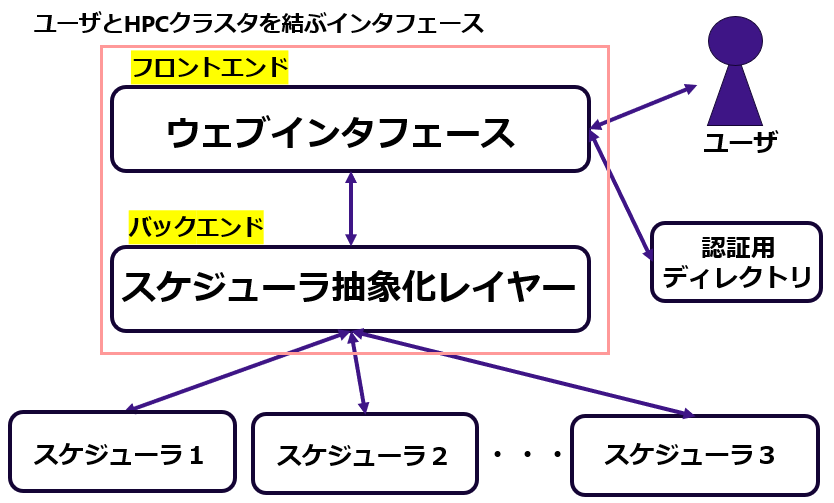
\includegraphics[width=75mm]{./fig/proposed_method.png}
  \caption{提案手法}
  \label{fig1}
\end{figure}

\section{評価}
ウェブ機能とスケジューラ抽象化機能をそれぞれ独立に実装し,連携させることでウェブインターフェスを介して様々なシステムを統一的に利用できる環境を実現する.そのために,ウェブ機能の基盤としてOOD,スケジューラ抽象化機能の基盤としてPSI/J\cite{citation_6}と呼ばれるPythonライブラリを利用し,両者を組み合わせることで提案手法を実装した.\par
本研究では,東北大学のスーパーコンピュータ「AOBA」で運用されているジョブスケジューラ(NEC Network Queuing System V, NQSV)がOODでサポートされていないという事実に着目して,NQSVをスケジューラ抽象化機能側に実装することと,それをウェブ機能側から利用できることを検証する.また,インタフェースをウェブ機能とスケジューラ抽象化機能に分けることで両者間の連携には実行時オーバヘッドが生じることが潜在的に懸念されるため,本実装におけるオーバヘッドを定量的に評価する.\par

\subsection{機能の実装}
実装環境として,OOD用のホストサーバと「AOBA」を想定したNQSVが使用されているHPCクラスタを用いて実装を行った.OODはログイン時に必要な認証用のディレクトリであるActive Directiory(AD)と連携して使用した.\par
始めにNQSVをスケジューラ抽象化機能側に実装した.PSI/Jはジョブの情報を格納するJobクラスとジョブの投入や削除などのメソッドをスケジューラごとにオーバーライドして定義しているJobExecutorクラスにより構成されている.今回は新たにNQSV用のJobExecutorクラスを作成し,ジョブの投入,削除,ステータス確認を行うための3つのメソッドを実装した.実装において,PSI/Jがサポートしている他のスケジューラ(Slumr, PBS Pro, LSF, Flux, Cobalt)はジョブの終了後にジョブのステータス(COMPLETED,CANCELED,FAILED)をコマンドの出力結果から確認できるが,NQSVではジョブの終了後にジョブのステータス(COMPLETED,CANCELED,FAILED)を確認できないという仕様上の問題があった.そのため,NQSVをサポートするにあたり,「ジョブ投入メソッド実行の有無」「ジョブ削除メソッドの実行の有無」「キュー内部のジョブの存在の有無」でジョブのステータスを判断するように修正した.ジョブは「ジョブ投入メソッドが実行され,キューにジョブが存在しない場合」にCOMPLETEDステータスとなる.また,「ジョブ削除メソッドの実行」によりCANCELEDステータスとなる.「ジョブ投入メソッドが実行され,キューにジョブが存在する場合」はQUEUEDステータスまたはACTIVEステータスとなる.今回適用した改修は,スケジューラが提供するジョブ管理のためのコマンドが,PSI/Jの想定している結果を返さない場合にも用いることができる.そのため,各ジョブスケジューラのコマンド出力に依らず,より汎用性の高い実装を行うことができたといえる.\par
続いて,ウェブ機能側であるOOD側からスケジューラ機能を用いることができるように実装する.実装における問題点として,OODがRubyで実装されていることに対して,PSI/Jはpythonで実装されているという点が挙げられる.そのため,Rubyスクリプト上でpythonライブラリを使用する必要がある.本実装ではPSI/Jを経由する際のオーバヘッドが小さく,単純な実装であるため,PSI/Jを用いたジョブの管理のためのpythonスクリプトをシェルを経由してRubyスクリプト上で直接実行する手法を用いた.この実装により,ウェブ機能としてOODを用いると,スケジューラ抽象化機能であるPSI/Jを経由して,指定したスケジューラにジョブの投入や削除を行うことができるようになった.また,PSI/Jを仲介することで,OOD未サポートであったNQSVでのジョブ管理をOOD上から操作することができるようになった.\par
図\ref{fig4}はOOD上でジョブを作成して投入・削除を行う「Job Composer」の画面である.ジョブを作成する際にクラスタをpsijに設定することで,psijを経由してSlurmクラスタやNQSVクラスタなど任意のHPCシステムにジョブの投入を行うことが確認できた.\par

\begin{figure}[h]
  \centering
  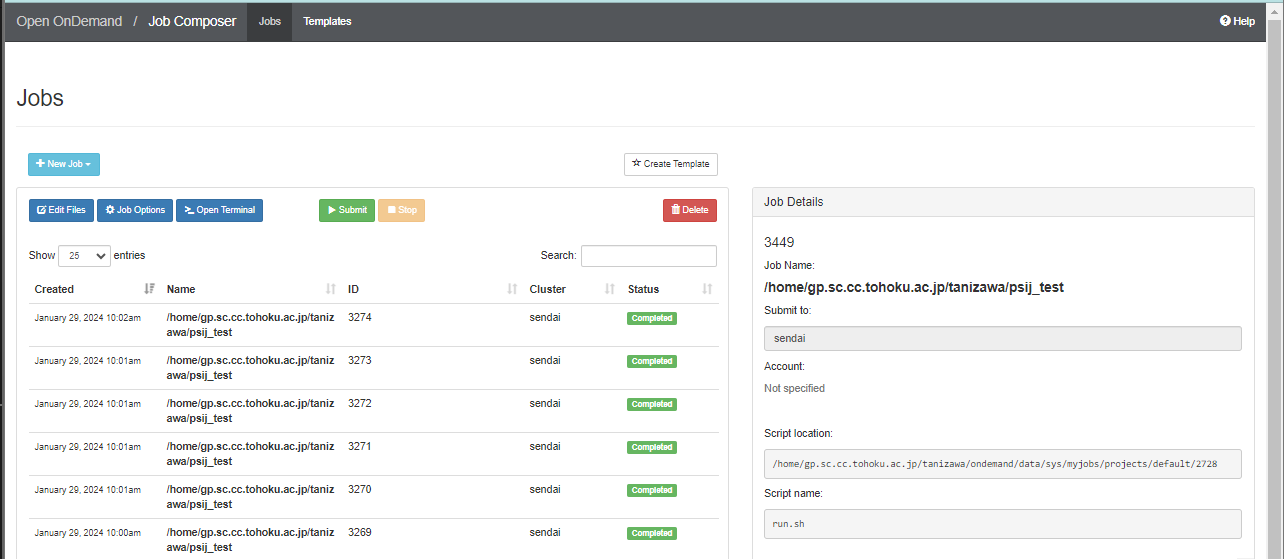
\includegraphics[width=75mm]{./fig/jobcomposer.png}
  \caption{Job Composerの画面}
  \label{fig4}
\end{figure}

\subsection{実行時オーバヘッド}
インタフェースをウェブ機能とスケジューラ抽象化機能に分けたことによる両者の連携時のオーバヘッドを測定する.実装において,シェルを介してpythonスクリプトを実行するため,その際のオーバヘッドの影響を評価した.測定は,seleniumと呼ばれるウェブページの自動制御ライブラリを用いて実行する.ローカルホストから別ホストのOODのポータルサイトにアクセスして,Job Composer画面でジョブの作成・投入を行う.ジョブの作成を開始した時刻から,投入したジョブが完了した時刻を計測してターンアラウンドタイムとする.ジョブの投入を1~10回連続で行い,そのターンアラウンドタイムを計測してPSI/Jを経由する時と経由しない時を比較した.以下の図\ref{fig2},図\ref{fig3}にその結果を示す.\par

\begin{figure}[h]
  \centering
  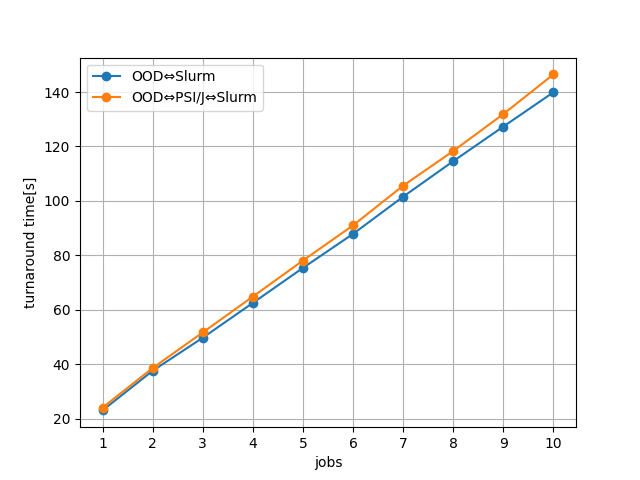
\includegraphics[width=75mm]{./fig/ave_1-20.png}
  \caption{実行時オーバーヘッドの比較}
  \label{fig2}
\end{figure}

\begin{figure}[h]
  \centering
  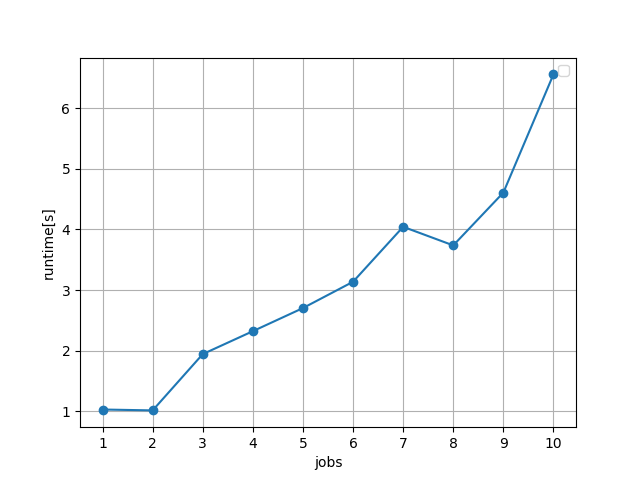
\includegraphics[width=75mm]{./fig/ave_diff_1-20.png}
  \caption{実行時オーバーヘッドの差}
  \label{fig3}
\end{figure}

計測は全部で20回行い,その平均値を使用して評価を行った.横軸は連続して投入したジョブの数,縦軸はジョブのターンアラウンドタイムを示している.図\ref{fig2}からPSI/Jを経由した提案手法の方がわずかにターンアラウンドタイムが大きいことがわかり,どちらの場合も連続投入したジョブの数に線形比例して増加している.また図\ref{fig3}から,ジョブの連続投入回数が多くなればなるほど両者の実行時オーバヘッドの差が大きくなっていることがわかる.\par
次に,ジョブの投入を0~100回連続投入した際の実行時オーバーヘッドを比較する.図\ref{fig5}は1~100回までジョブの連続投入数を10回ずつ増やしたときのターンアラウンドタイムの比較を示した.1~10回の連続投入の場合と同じく,PSI/Jを経由した場合の方がわずかにターンアラウンドタイムが大きくなっており,連続投入するジョブ数を大きくしても極端にオーバヘッドに差が出ることはなく同様の傾向が見られることがわかった.\par

\begin{figure}[h]
  \centering
  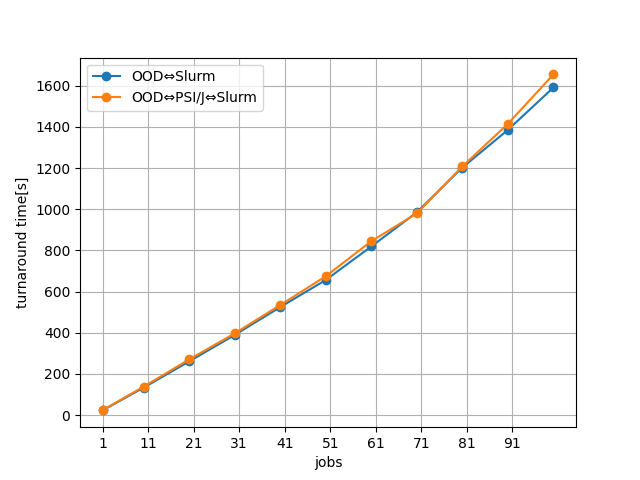
\includegraphics[width=75mm]{./fig/100jobs.png}
  \caption{ジョブ数を増加した際のオーバヘッドの比較}
  \label{fig5}
\end{figure}

\section{考察}
検証の結果,OODのインタフェースからNQSVを利用してジョブの投入や削除が行われることが確認された.ただし、ジョブのホールドとリリースに関する機能は、OODでは実行されているがPSI/Jでは未実装であるという課題もある.また,ウェブ機能とスケジューラ抽象化機能に分離する前と後で指定数のジョブを連続投入してスループットを比較した.ジョブ数が1~10の範囲内であれば,両者の差が最大でも5\%を超えないことから,提案手法によって生じるオーバヘッドは十分に小さいことが明らかになった.\par


\section{結論}
ウェブインタフェースを介してHPCシステムを利用する環境をウェブ機能とスケジューラ抽象化機能に分離することにより,それぞれの機能を独立に開発していくことが可能となった.それによってソフトウェアの保守性を高めることが可能となり,長期にわたって多様なシステムをサポートしていく労力の削減効果が期待できる.また,機能分離に伴う実行時オーバヘッドは無視できる程度であり,運用上の問題にはならないことが明らかになった.今後の課題として,PSI/Jにジョブ管理の他のメソッドを追加することでOODで実行できる機能を増やすこと,OODではサポートされていない他のジョブスケジューラをPSI/Jを経由して実装することなどが挙げられる.\par



\bibliographystyle{junsrt}
\bibliography{refer}

\end{document}